\chapter{METHODOLOGIES ET MODELES}
\thispagestyle{empty}

\section{Pipeline general}

Le projet suit une logique en trois couches. D'abord, le graphe Wiki-CS est
enrichi avec le texte reel des articles et des metadonnees. Ensuite, plusieurs
familles de representations sont calculees sur ce graphe. Enfin, ces
representations sont evaluees dans des experiences de recommandation hors ligne
et exposees a travers une interface applicative locale.

\begin{figure}[H]
\centering
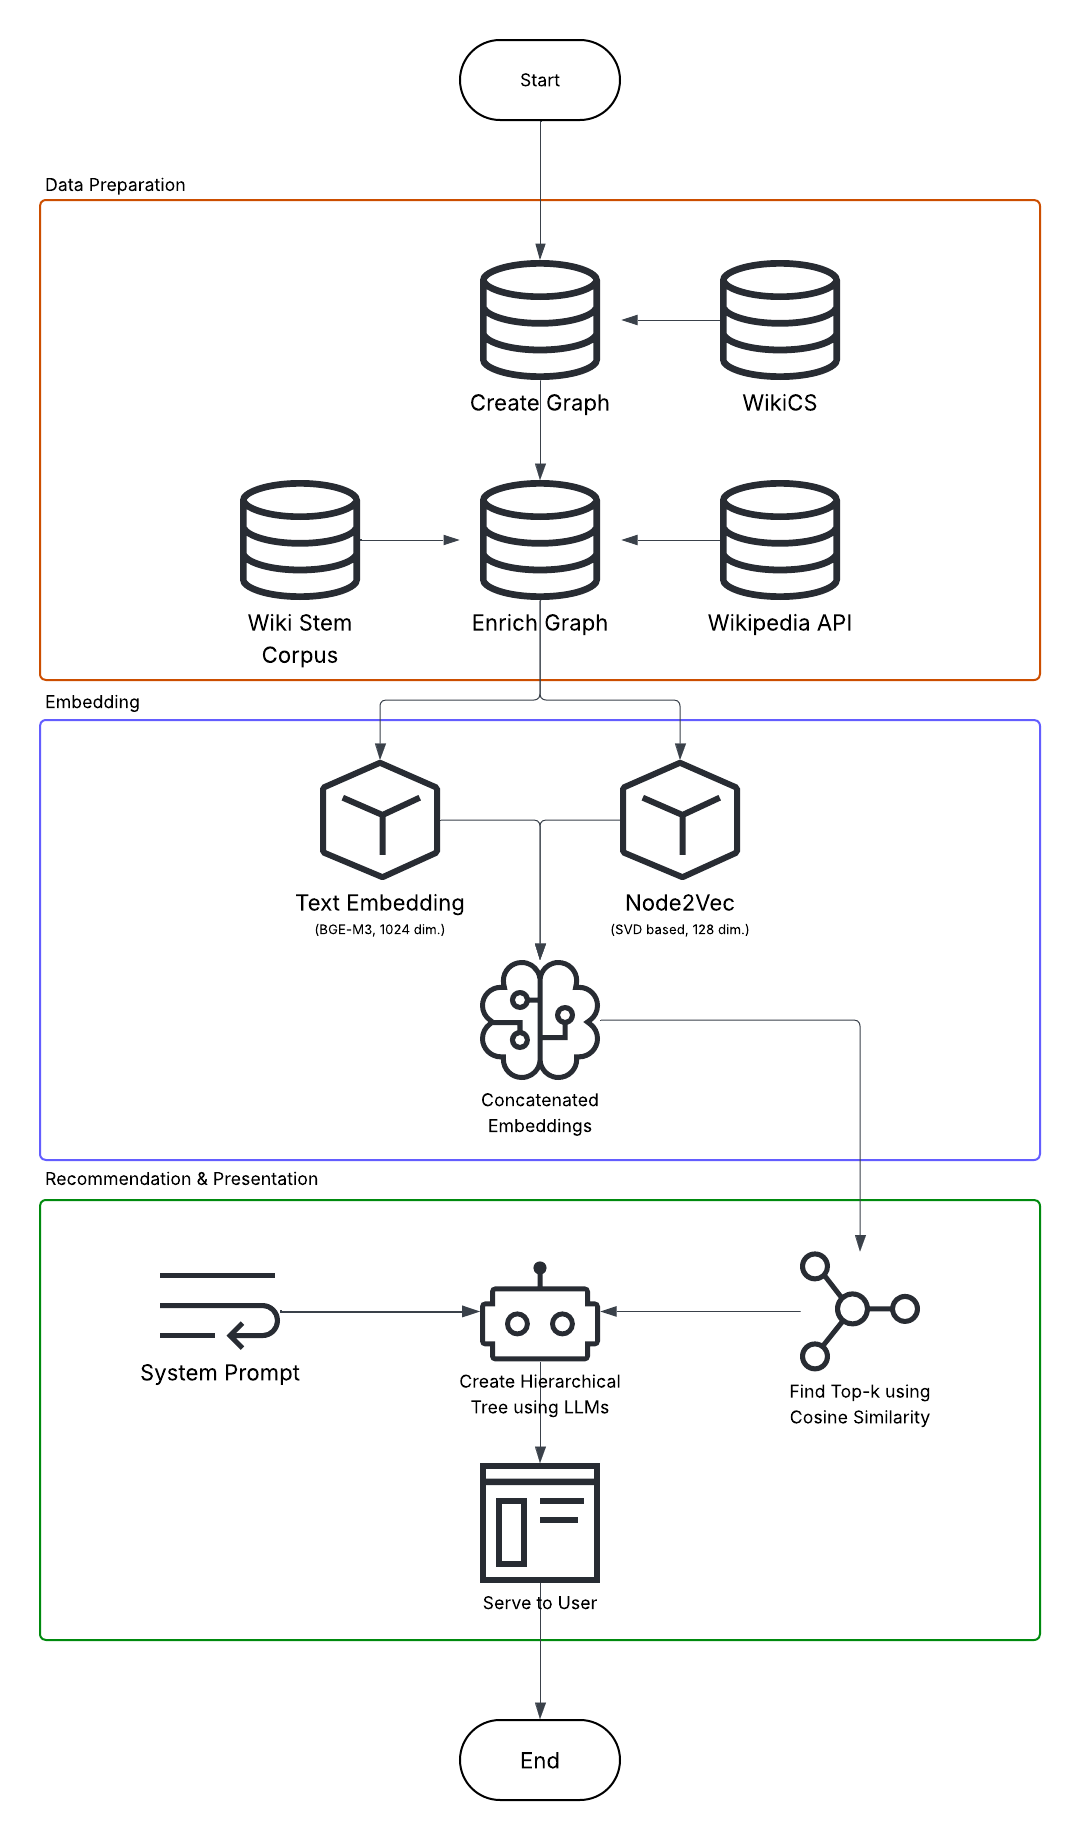
\includegraphics[width=0.82\textwidth]{figures/architecture.png}
\caption{Architecture conceptuelle du pipeline du projet, de la creation du graphe a la recommandation puis a une presentation future en parcours d'apprentissage.}
\label{fig:final-architecture}
\end{figure}

La Figure~\ref{fig:final-architecture} doit etre lue comme une feuille de route
conceptuelle du projet. Elle represente l'interaction visee entre la
preparation des donnees, la generation des embeddings, la recommandation et la
presentation, meme si la couche d'organisation mise en oeuvre a evolue au cours
du temps.

\section{Construction du jeu de donnees}

L'ossature topologique brute provient de Wiki-CS~\cite{mernyei2020wikics}. Le
projet rehydrate ensuite les noeuds avec le texte reel des articles Wikipedia
et stocke l'ensemble de travail obtenu dans l'espace Custom-WikiCS. Les
statistiques stables du graphe utilisees dans les rapports ulterieurs sont:
\begin{itemize}
    \item noeuds initiaux: 11,701;
    \item noeuds isoles retires: 334;
    \item noeuds actifs apres nettoyage: 11,367;
    \item aretes orientees: 291,039;
    \item aretes non orientees: 216,123.
\end{itemize}

Cette etape d'enrichissement transforme le benchmark initial en un espace de
recommandation: les noeuds ne sont plus seulement des identifiants
structurels, mais des objets articles avec titres, texte, liens et contenu
pret pour la generation d'embeddings.

\section{Familles de representations}

\subsection{Representation semantique}

La representation semantique principale utilise les embeddings textuels
BGE-M3~\cite{chen2025bgem3}. Chaque article est encode sous la forme d'un
vecteur de dimension 1024. Ces embeddings permettent une recuperation
semantique directe par similarite cosinus et constituent egalement l'une des
deux moities des modeles hybrides. Des travaux exploratoires anterieurs
incluaient une autre famille d'embeddings textuels, mais les rapports plus
tardifs convergent vers BGE-M3 comme representation semantique principale.

\subsection{Representation structurelle}

Le volet structurel du projet a evolue au fil des etapes. Les premieres
experiences comprenaient une approximation de Node2Vec a base de SVD, adaptee
au CPU. Les experiences ulterieures se sont orientees vers un cache structurel
Node2Vec dedie, aligne sur le decoupage d'evaluation corrige. Deux variantes
sont conservees:
\begin{itemize}
    \item Node2Vec non corrige;
    \item Node2Vec corrige, avec application d'une penalite de degre de type
    loi de puissance.
\end{itemize}

Dans le cadre d'evaluation corrige, le coefficient structurel de loi de
puissance estime est
$\alpha_{\text{structural}} \approx 2.9966$.

\subsection{Baselines par reseaux de neurones sur graphes}

Deux baselines structurelles par GNN sont implementees:
\begin{itemize}
    \item GCN~\cite{kipf2017semi},
    \item GraphSAGE~\cite{hamilton2017inductive}.
\end{itemize}

Ces modeles sont entraines comme baselines structurelles plutot que comme
modeles textuels semantiques. Ils sont importants pour la comparaison car ils
apprennent directement des representations de noeuds a partir de la structure
du graphe, au lieu de s'appuyer sur des embeddings Node2Vec fixes.

\subsection{Modeles hybrides et fusion}

Le projet compare plusieurs manieres de combiner les signaux semantiques et
structurels:
\begin{itemize}
    \item la concatenation directe de BGE-M3 et de Node2Vec;
    \item la concatenation corrigee avec Node2Vec penalise par le degre;
    \item des modeles hybrides avec pooling, dans lesquels BGE-M3 est reduit de
    1024 a 128 dimensions avant concatenation;
    \item une fusion par reciprocal rank entre GCN et BGE-M3.
\end{itemize}

Ces alternatives sont importantes parce que la conception de la fusion s'est
revelee tres sensible. La concatenation brute, la concatenation corrigee, les
hybrides avec pooling et la fusion au niveau du rang ne se comportent pas de la
meme maniere a l'evaluation.

\section{Interface applicative}

Le prototype local n'est plus seulement une maquette. Il expose une recherche
active, la selection de modele, la recuperation classee et la previsualisation
d'articles a partir des artefacts mis en cache du projet.

\begin{figure}[H]
\centering
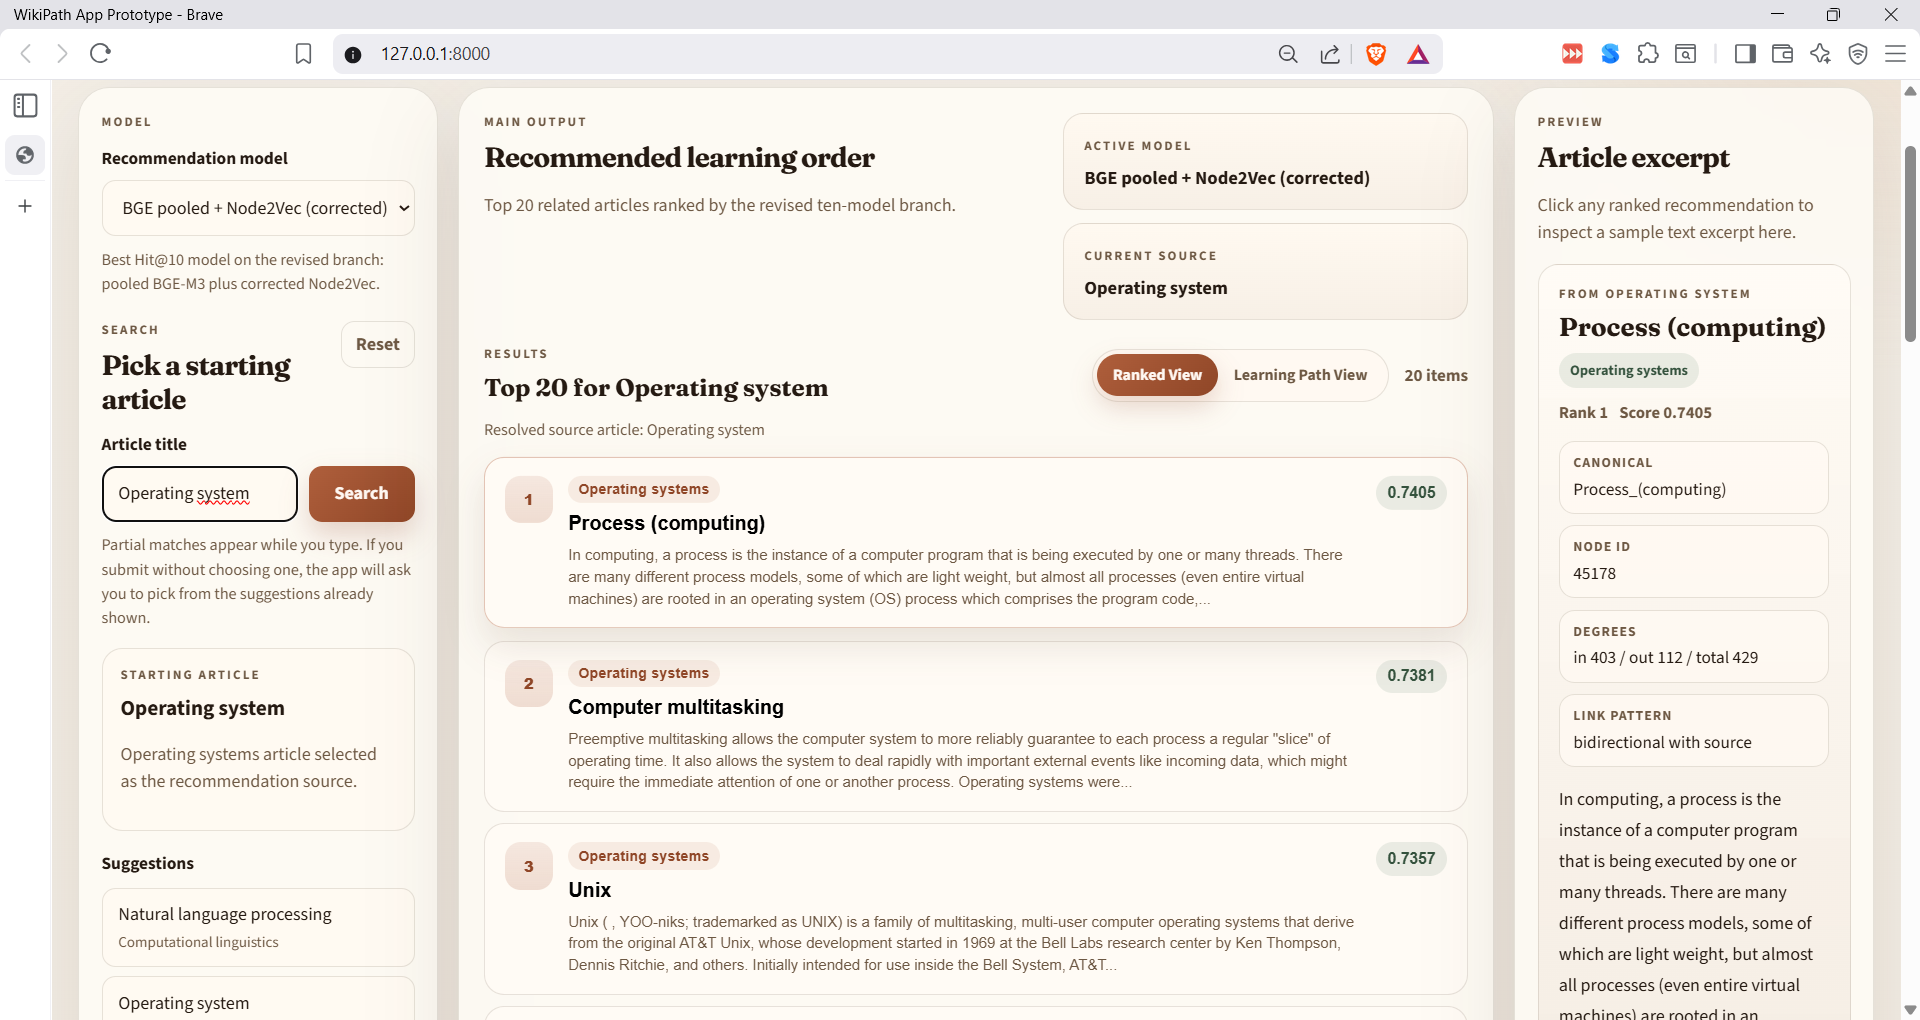
\includegraphics[width=\textwidth]{figures/query-and-results.png}
\caption{Interface implementee en vue classee du prototype local WikiPath.}
\label{fig:final-ui-ranked}
\end{figure}

\begin{figure}[H]
\centering
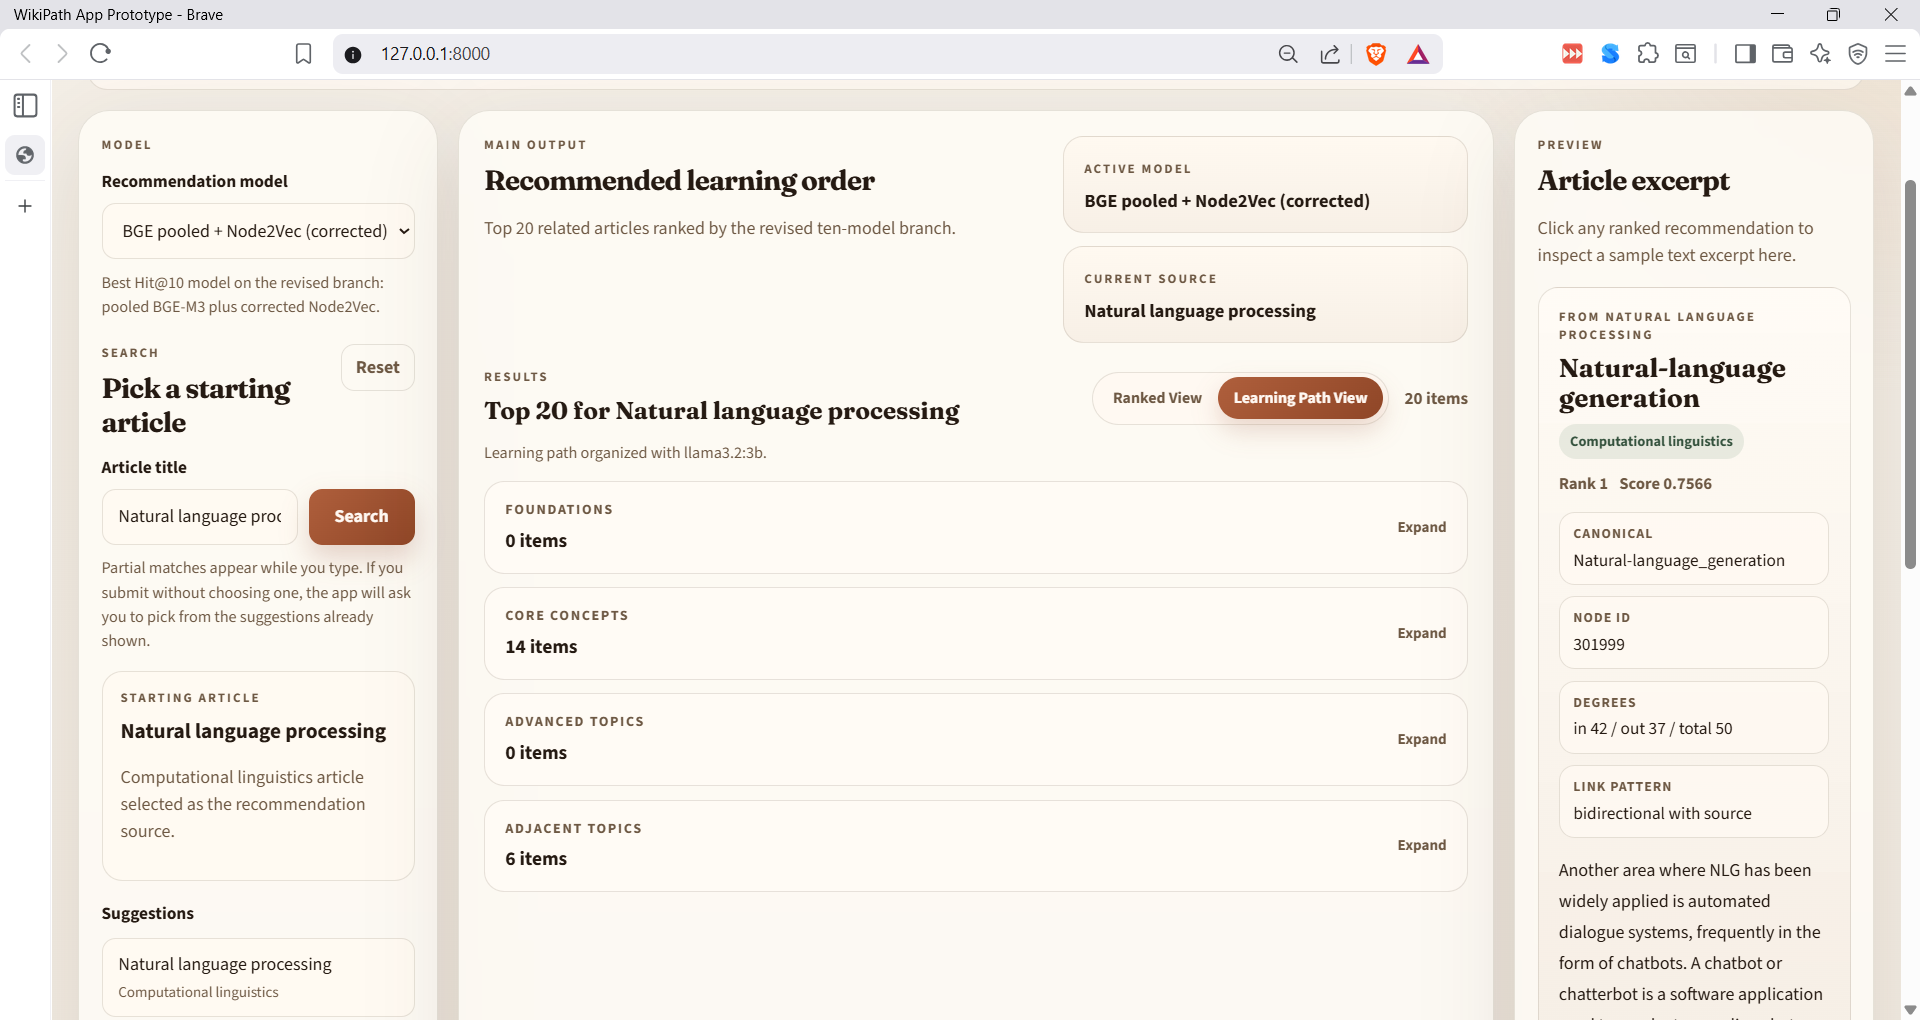
\includegraphics[width=\textwidth]{figures/path-result.png}
\caption{Vue de type parcours d'apprentissage du prototype actuel. L'ensemble classe des resultats est reorganise en sections pour la presentation.}
\label{fig:final-ui-path}
\end{figure}

L'interface remplit deux roles. D'une part, elle sert d'outil d'inspection
qualitative pour la famille de modeles. D'autre part, elle rend le systeme de
recommandation concret au-dela des seuls tableaux de notebooks.

\section{Evolution de la couche LLM}

La couche de parcours d'apprentissage a fortement evolue pendant le projet.
Durant la periode des rapports intermediaires, l'idee etait d'utiliser un
petit modele local via Ollama. Cette approche etait attractive car elle
preservait une execution entierement locale, mais elle s'est revelee fragile
en pratique pour l'organisation structuree d'un ensemble complet de
recommandations top-20. Les sorties etaient frequemment mal formees, faibles
sur le plan semantique ou trop fortement regroupees dans un petit nombre de
categories.

L'application actuelle utilise donc une strategie differente. La recuperation
et le classement restent locaux et s'appuient sur les artefacts du projet mis
en cache, mais l'organisateur optionnel utilise desormais un appel Gemini a
sortie structuree sur les titres deja recuperes. Le backend verifie que:
\begin{itemize}
    \item seuls les titres fournis par la recuperation sont utilises;
    \item chacun apparait exactement une fois;
    \item l'ordre de classement initial est preserve.
\end{itemize}

Si la sortie structuree echoue a la validation, l'application revient a un
parcours heuristique. Cette refonte est importante: le LLM est desormais traite
comme un organisateur contraint et non comme un generateur de candidats de
recommandation.

\section{Protocole d'evaluation}

Le rapport final utilise comme cadre canonique un protocole revise
d'evaluation structurelle non orientee. Les principales statistiques du
decoupage de phase 0 sont les suivantes:
\begin{itemize}
    \item aretes structurelles non orientees totales: 216,123;
    \item aretes d'apprentissage: 172,900;
    \item aretes de test: 43,223;
    \item paires d'evaluation etendues: 86,446;
    \item noeuds d'evaluation: 9,022.
\end{itemize}

Chaque arete de test non orientee $\{u,v\}$ est developpee en deux requetes
d'evaluation orientees, $u \rightarrow v$ et $v \rightarrow u$, pour les
metriques de classement. Les metriques de qualite de recommandation sont
ensuite calculees sur des listes top-20. Les extensions ulterieures reutilisent le meme cadre d'evaluation et n'etendent que la
couche de mesure, sans reconstruire le decoupage structurel.
